\documentclass[letter]{article}
\usepackage[margin=1in]{geometry}
%\documentclass[10pt]{article}
\usepackage[final]{graphicx}
\usepackage{color}


%\usepackage[cm]{fullpage}
\usepackage{
amsfonts,amssymb,
amsmath,
url,graphics,subfig,
cite,
calc,
psfrag, bm,
amsthm, 
paralist}

%\renewcommand{\textwidth}{5.5in}

%---- Some math. macro
\newcommand\infsum[1][n]{\ensuremath{\sum_{#1=-\infty}^\infty}}

% Here's the definition of Sb, stolen from amstex
    \makeatletter
    \def\multilimits@{\bgroup
  \Let@
  \restore@math@cr
  \default@tag
 \baselineskip\fontdimen10 \scriptfont\tw@
 \advance\baselineskip\fontdimen12 \scriptfont\tw@
 \lineskip\thr@@\fontdimen8 \scriptfont\thr@@
 \lineskiplimit\lineskip
 \vbox\bgroup\ialign\bgroup\hfil$\m@th\scriptstyle{##}$\hfil\crcr}
    \def\Sb{_\multilimits@}
    \def\endSb{\crcr\egroup\egroup\egroup}
\makeatother

\newtheoremstyle{t}         %name
    {\baselineskip}{2\topsep}      %space above and below
    {\rm}                   %Body font
    {0pt}{\bfseries}  %Heading indent and font
    {}                      %after heading
    { }                      %head after space
    {\thmname{#1}\thmnumber{#2}.}

\theoremstyle{t}
\newtheorem{q}{Q}
\parindent=0pt 

\begin{document}

\setcounter{page}{1}
\linespread{1.1}
\normalsize

\setlength{\parskip}{.2cm}

\begin{center} {\Large \textbf{
ECS289F Progress report\vspace{.2cm} \\ --- Opinion Dynamics with  reluctant agents ---}} \vspace{.3cm}

{Hoi-To Wai, Christopher Patton}

\today

\end{center}
\vspace{0.1cm}


% \begin{abstract}
%This note is a summary of the rudimentary ideas I have for ECS289F's project. Specifically, I will propose a model for the opinion dynamics with reluctant agents, i.e., agents who are reluctant to blend their idea with his/her neighbors. Explorations into the Bitcoin attack model will also be investigated. (For the references cited here, I believe that better references must exists, but I will need to spend more time on mining them.)
%\end{abstract}


%-----------------------------------------------------------------------------
%\vspace{0.5cm}

%\section{Introduction} \vspace{-.3cm}
This document reports on the recent progress we have made for the course project in the two weeks after the project proposal's submission. The goal of this project is to consider a new aspect for the DeGroot's model by considering an opinion dynamic model where a subset of agents are \emph{reluctant} to update their opinion. 

%The idea of modeling opinion dynamics has been pioneered by DeGroot \cite{Degroot_74}. He proposes a simple model of social interactions in which both the time it will take to reach consensus, as well as the consensus score itslf, can be computed easily. Though this model has proven to be insightful in this domain, it doesn't capture the dynamics of many consensus scenarios. Namely, we would like to capture the throughput and latency dynamics of censor networks. 

Let us first recap on the system model.
We consider an undirected graph $G = (V,E)$ with $|V| = n$. Each agent $i \in V$ holds an initial opinion ${\bm w}_i^{(0)} \in \mathbb{R}^L$. At time $k$, the agents exchange their beliefs with the others to compute:
\begin{equation}\label{eq:op}
\hat{\bm w}_i^{(k)} = \sum_{j \in \mathcal{N}_i} P_{ij}^{(k)} {\bm w}_j^{(k-1)},
\end{equation}
where $0 \leq P_{ij}^{(k)} \leq 1$ models the trust agent $i$ has on agent $j$ at time $k$. Importantly, we assume $\sum_{j=1}^{|V|} P_{ij}^{(k)} = 1$ and $\sum_{i=1}^{|V|} P_{ij}^{(k)} = 1$. Notice that the matrix ${\bm P}^{(k)}$ is time-variant. 

The vector $\hat{\bm w}_i^{(k)}$ is the opinion that agent $i$ is supposed to hold at time $k$. In DeGroot's model, the agents are updating instantly such that ${\bm w}_i^{(k)} = \hat{\bm w}_i^{(k)} $. In this case, it is known that ${\bm w}_i^{(k)}$ converges to the average of $\{{\bm w}_i^{(0)} \}$ asymptotically, i.e., achieving the `wisdom of the crowd',  under some mild assumptions. 
However, in our model, some agents are reluctant such that they don't update \emph{immediately}. Instead, ${\bm w}_i^{(k)}$ is updated by:
\begin{equation} \label{eq:adapt}
{\bm w}_i^{(k)} = \frac{c_i^{(k)}}{\tau_i} \hat{\bm w}_i^{(k - c_i^{(k)} + 1)} + \frac{\tau_i - c_i^{(k)}}{\tau_i} {\bm w}_i^{(k-c_i^{(k)})},~i \in V_r,
\end{equation}
where $V_r \subseteq V$ is the set of reluctant agents and 
\[
c_i^{(k)} = \begin{cases}
1 &,~{\rm if}~P_{ij}^{(k)} \neq 0,~\text{for some}~j \in V~\text{(agent $i$ talked at time $k$)}. \\
\min\{ c_i^{(k-1)} + 1, \tau_i \} &,~{\rm otherwise}.
\end{cases}
\]
is a counter variable and $\tau_i \in \mathbb{Z}$ is the adaptation rate of $i$. In other words, the reluctant agent will slowly adapt to the new opinion in $\tau_i$ time steps. Notice that the `normal' agents are special case of this with $\tau_i = 1$. 

\section{(Preliminary) Convergence Analysis} 
In this section, we perform a convergence analysis for the proposed opinion dynamics model based on \cite{}. The main result is that we have proved that the opinions will  converge to a (biased) consensus with high probability. As a preliminary observation, we found that the converged opinion will be biased towards the initial opinions of the reluctant agent in expectation. 

We found that our proposed model can be analyzed under the framework of \cite{}, which studied a delayed consensus model. In the analysis, the main idea is to consider an augmented system with a few extra nodes proportional to the maximum delay allowed in the system. As the augmented system is delay-free, it can subsequently be analyzed using the available tools. 

Let us apply the above approach to our model. We consider a directed graph $G' = (V',E')$ where $V'$ contains all the nodes from $V$ together with a few augmented node, defined as follows. For each $i \in V_r$, we define $1 + 2(\tau_i - 1)$ new nodes denoted by $\{ i' \} \cup \{i + N, ..., i + (\tau_i-1)N\} \cup \{ i'+N, ..., i' + (\tau_i-1)N\}$. Here, the $i'$th node stores the value of $\hat{\bm w}_i^{(k)}$. The nodes $\{i + N, ..., i + (\tau_i-1)N\}$ and $\{ i'+N, ..., i' + (\tau_i-1)N\}$ stores the delayed version of ${\bm w}_i$ and $\hat{\bm w}_i$, respectively. The inter-connectivity of these nodes are best illustrated by the example in Fig.~\ref{fig:augment}. 

\begin{figure}[t]
\centerline{\resizebox{.55\textwidth}{!}{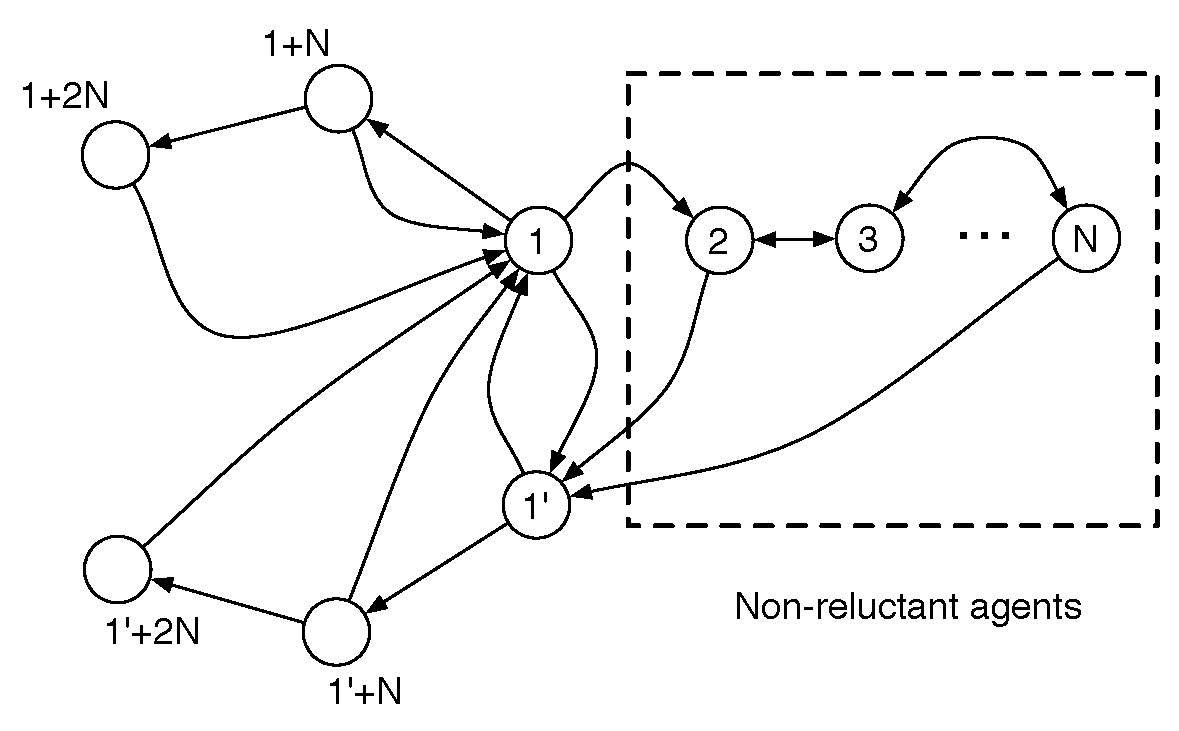
\includegraphics{./augmented_graph}}
}
\caption{The circuit model for the $(i,k)$ branch.
} \label{fig:augment}
\end{figure}

\section{(Preliminary) Simulation Studies}


%We will study how the reluctant agent will affect the consensus result in the model. In the first stage, we will examine (via simulation) the bias introduced by adding reluctant agents. How do topological properties, such as degree distribution, betweenness, and centrality impact the bias? and what about the speed of convergence? These questions will be addressed both analytically and empirically with respect to a few rew relevant network models discussed in class. A concrete result of this work will be a suite of tools for simulating various consensus scenarious on hand of real as well as synthetic data. 
%
%As an extension, we will study if we can recover the `wisdom of the crowd' given that we know some agents are reluctant. Another possible extension will be to consider discrete opinion dynamics. \vspace{-.2cm}
%
%\subsection{Previous works and references} 
%Our work is based upon the pioneering paper by DeGroot \cite{Degroot_74} and a recent survey in \cite{Fagnani2014}. Furthermore, the reluctant agent model is inspired by \cite{Acemoglu2013}, which studies the effect of \emph{stubborn} agents in a social network. For the simulation, we may also follow the reference \cite{Das2014} which has conducted experiments on opinion dynamics using real data. 


%\renewcommand{\refname}{\vspace{-1.5cm}}
%\small
\bibliographystyle{IEEEtran}
\bibliography{paper}


\end{document}
